\documentclass{article}
\usepackage{graphicx}
\usepackage{epstopdf}

\begin{document}
\begin{figure}\centering
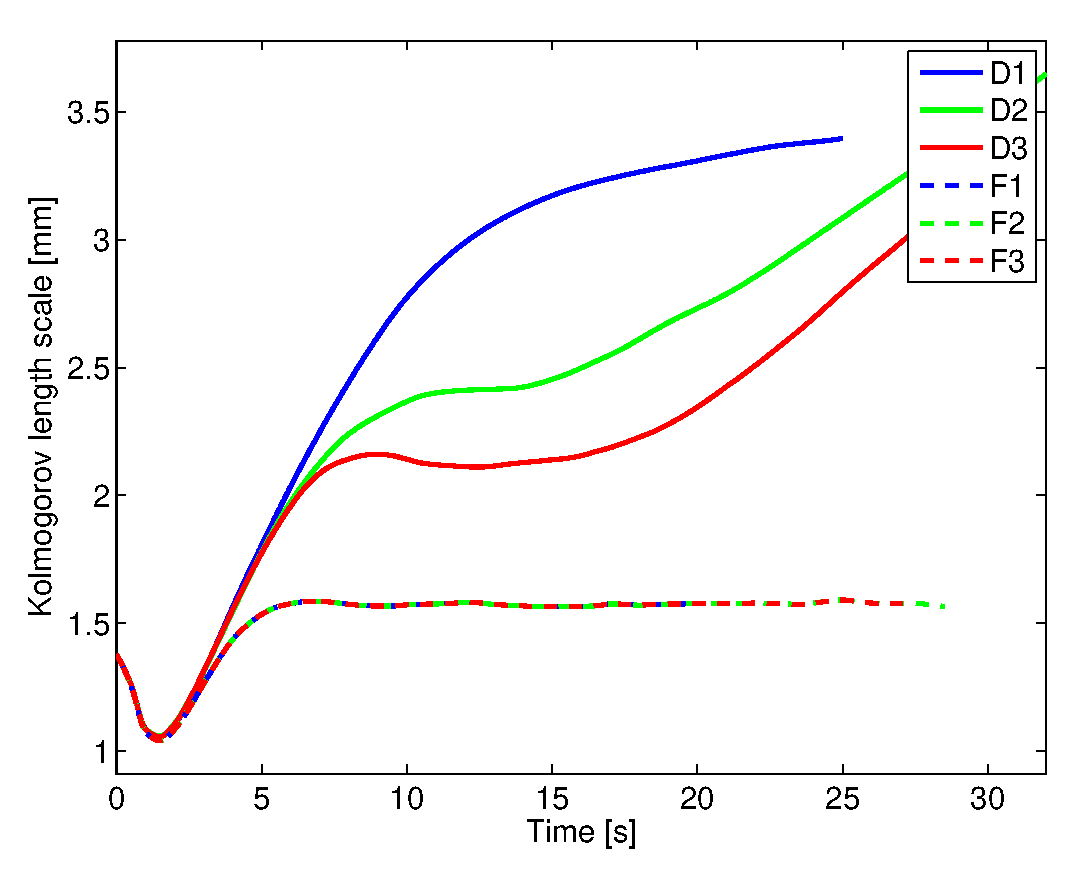
\includegraphics[width=\textwidth]{Figures/eta}
\caption{Temporal change of the Kolmogorov length scale for the six simulation
scenarios. See main text for the detail on the different scenarios.}
\end{figure}

\begin{figure}\centering
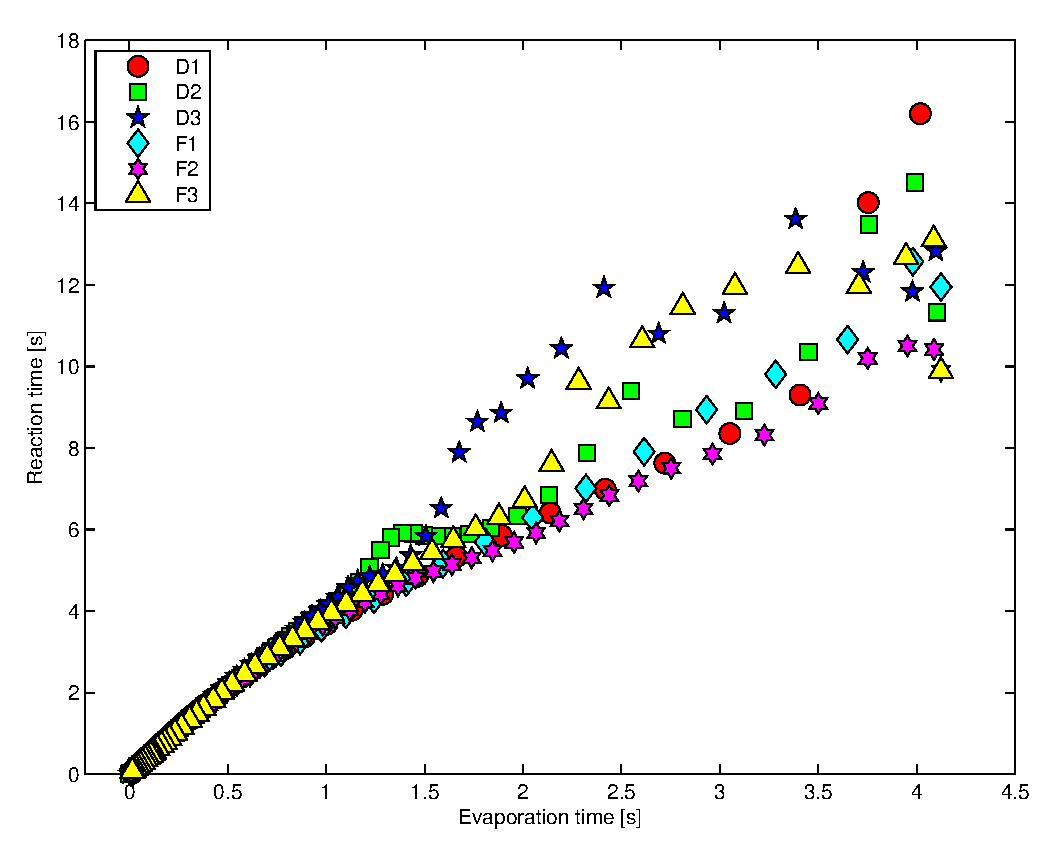
\includegraphics[width=0.49\textwidth]{Figures/tevap_treact}
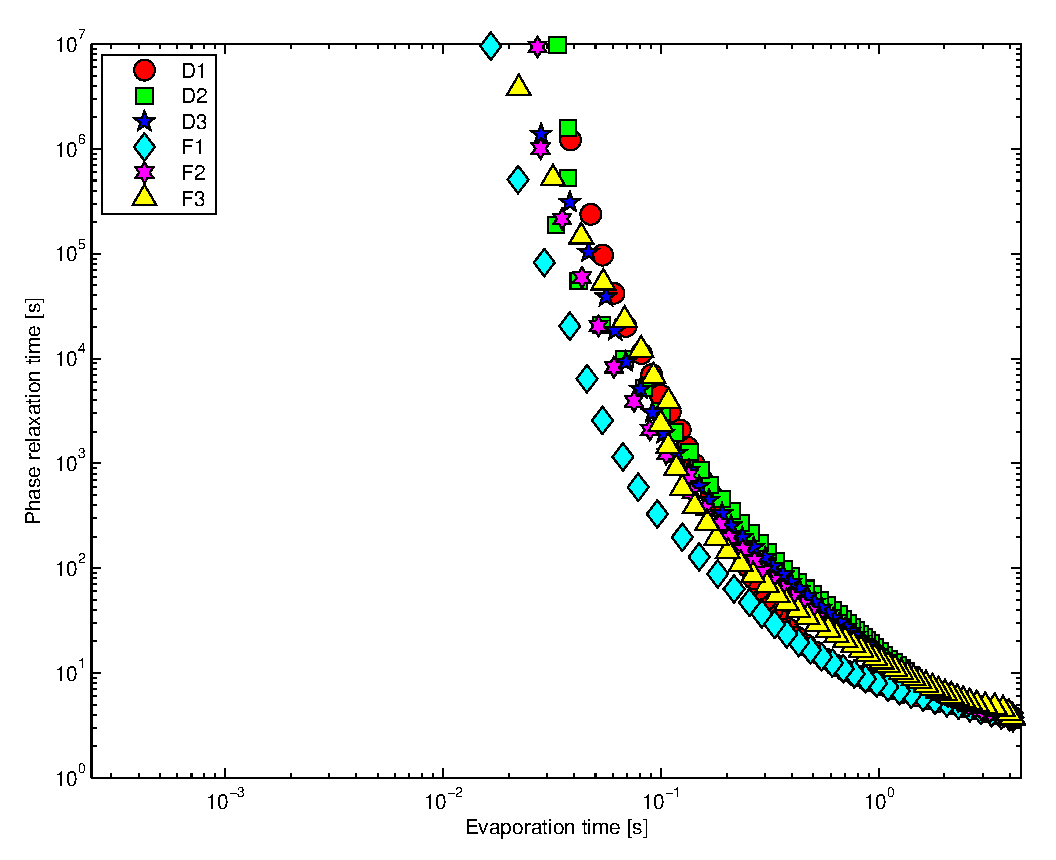
\includegraphics[width=0.49\textwidth]{Figures/tevap_tphase}
\caption{Relationship of evaporation time to reaction time (a) and phase relaxation time
(b). Each point represents an instantaneous domain mean; different color denotes the six
different scenarios.}
\end{figure}

\begin{figure}\centering
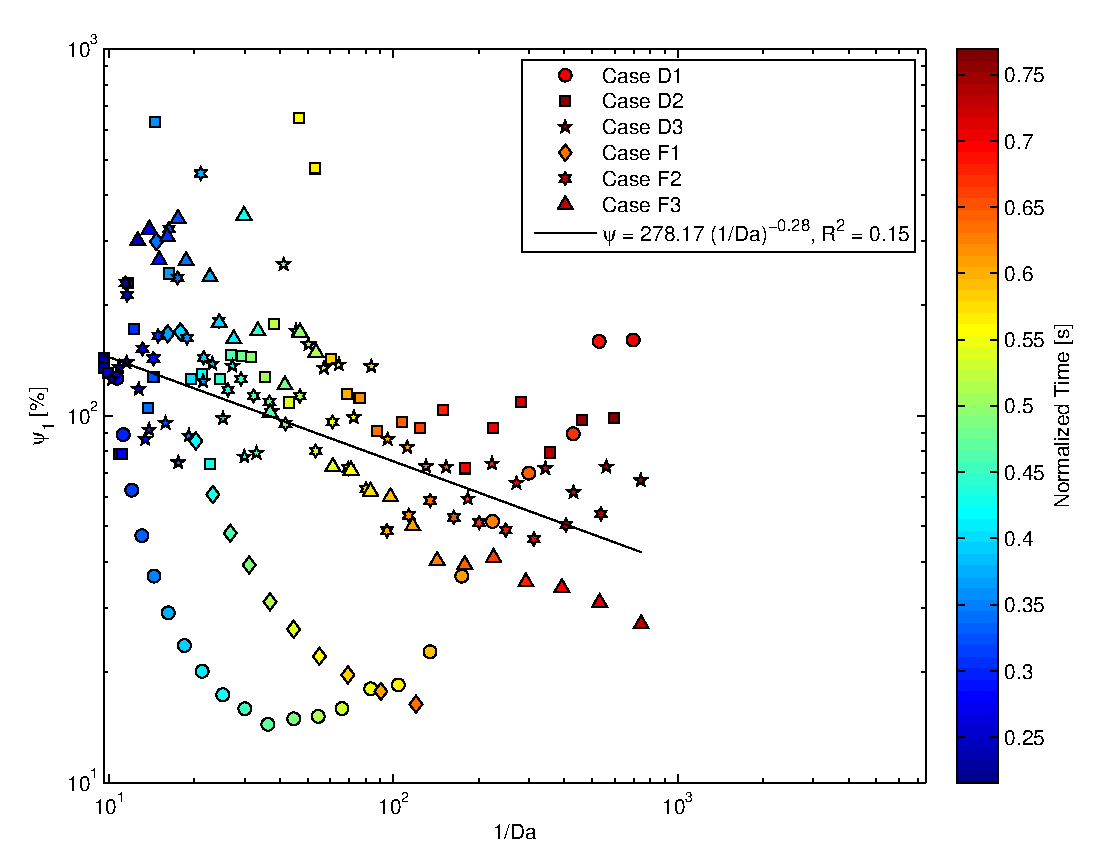
\includegraphics[width=0.49\textwidth]{Figures/phi1da_phase}
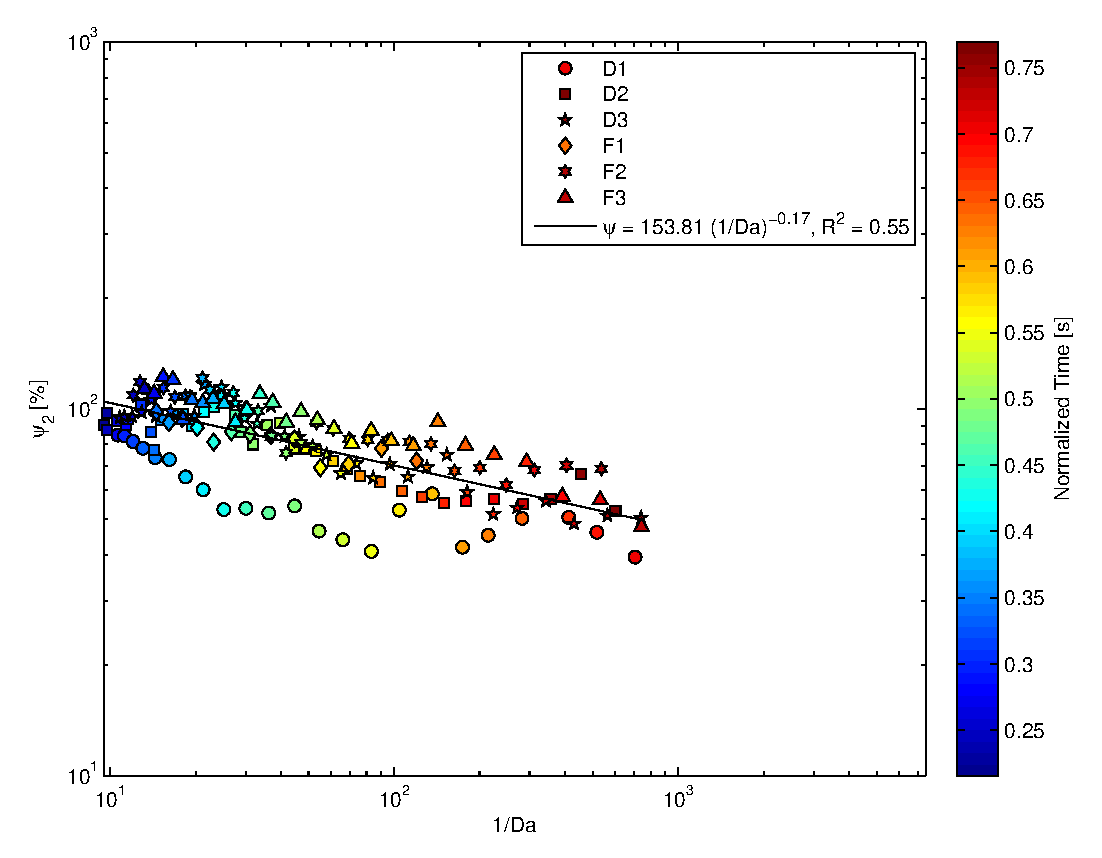
\includegraphics[width=0.49\textwidth]{Figures/phi2da_phase}\\
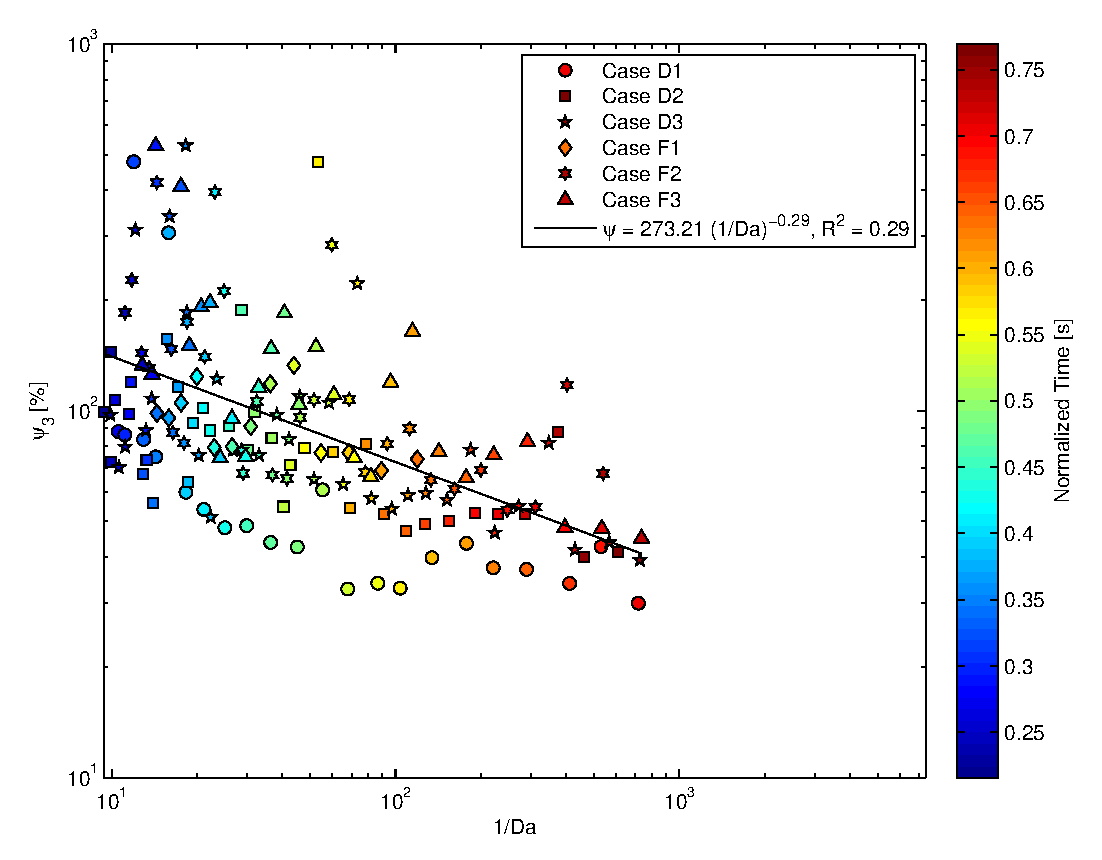
\includegraphics[width=0.49\textwidth]{Figures/phi3da_phase}
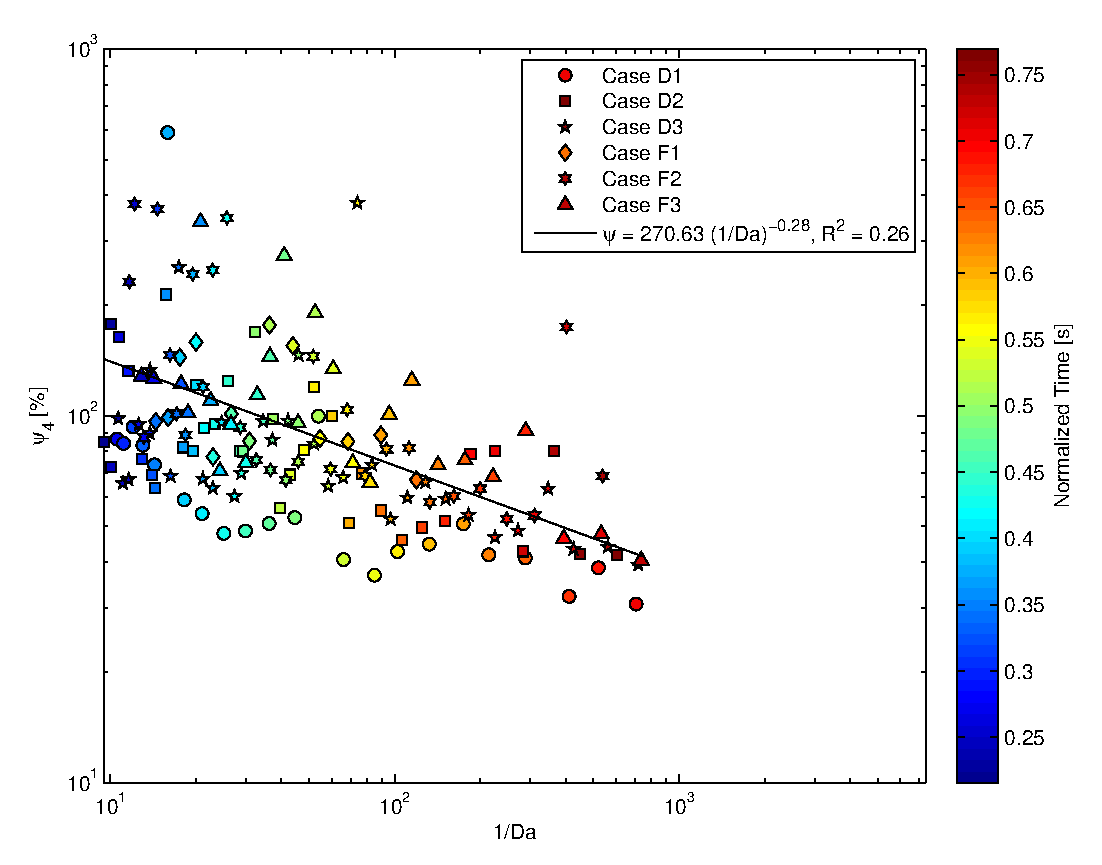
\includegraphics[width=0.49\textwidth]{Figures/phi4da_phase}\\
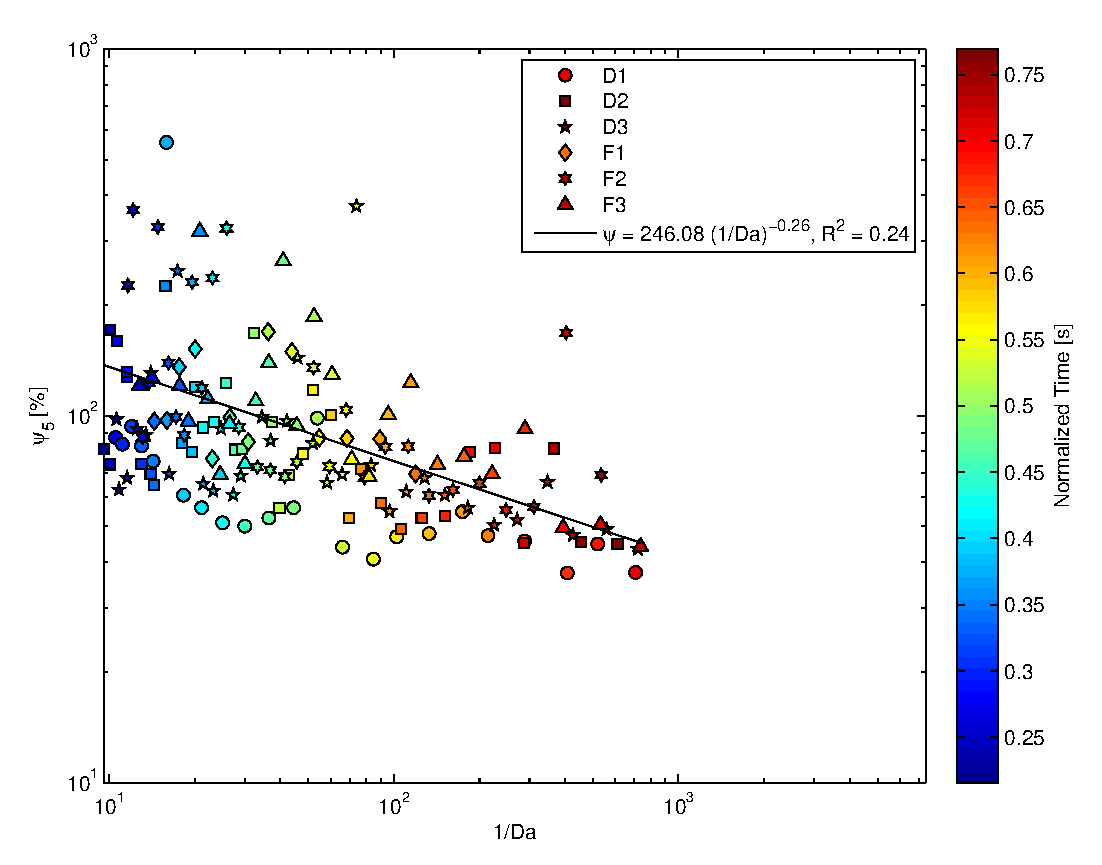
\includegraphics[width=0.49\textwidth]{Figures/phi5da_phase}
\caption{Same as Figure 8 in the main text, but the Damköhler number Da is based on the
phase relaxation time.}
\end{figure}

\begin{figure}\centering
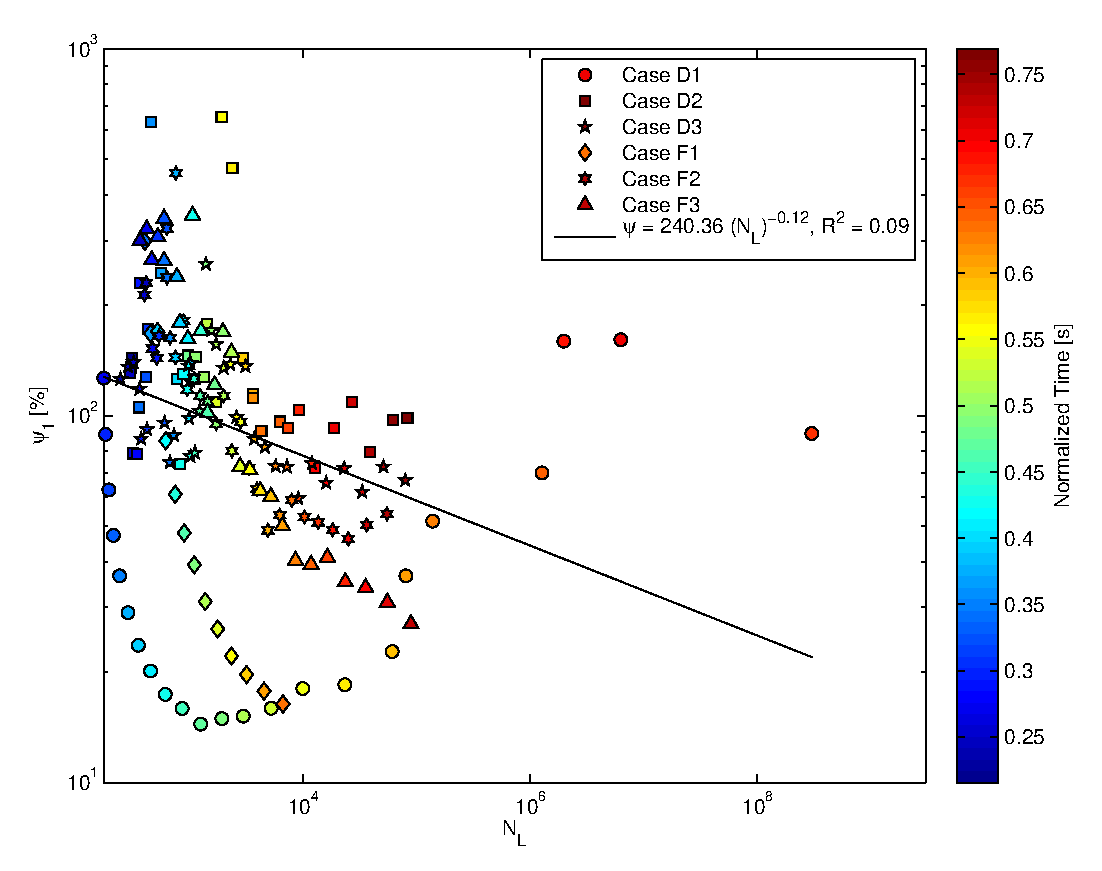
\includegraphics[width=0.49\textwidth]{Figures/phi1nl_phase}
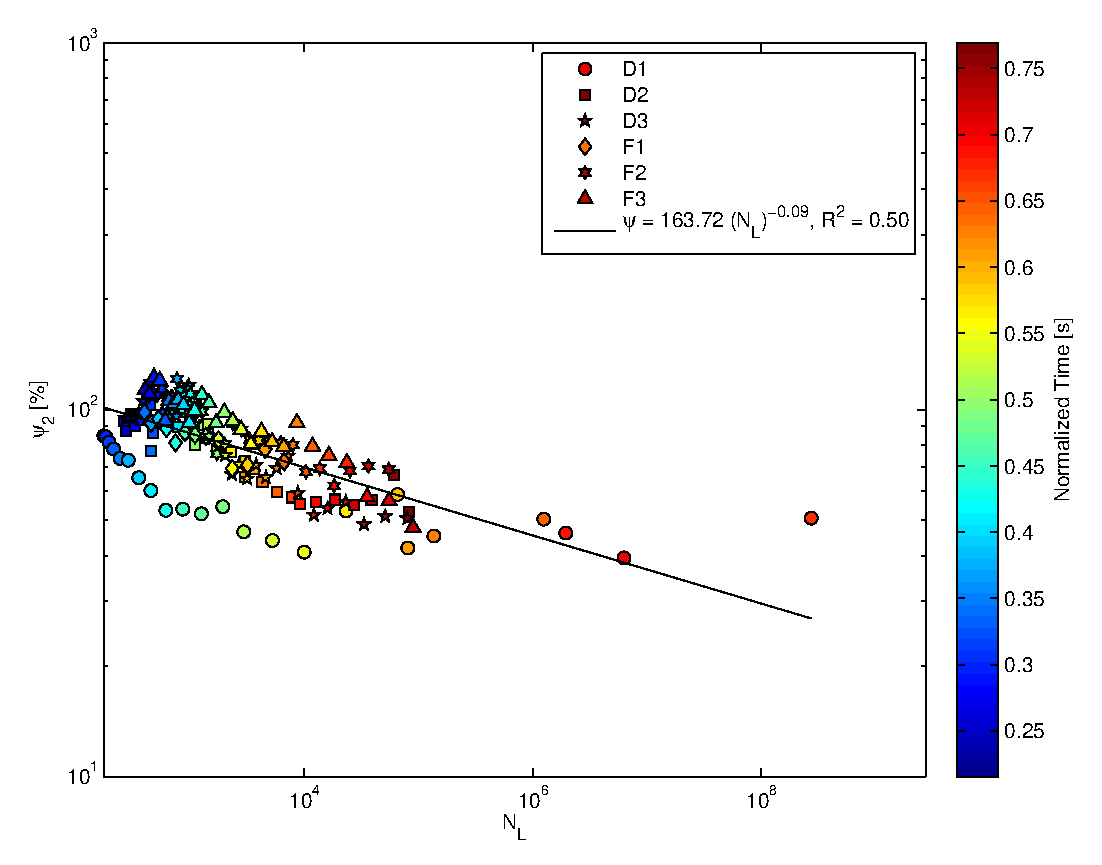
\includegraphics[width=0.49\textwidth]{Figures/phi2nl_phase}\\
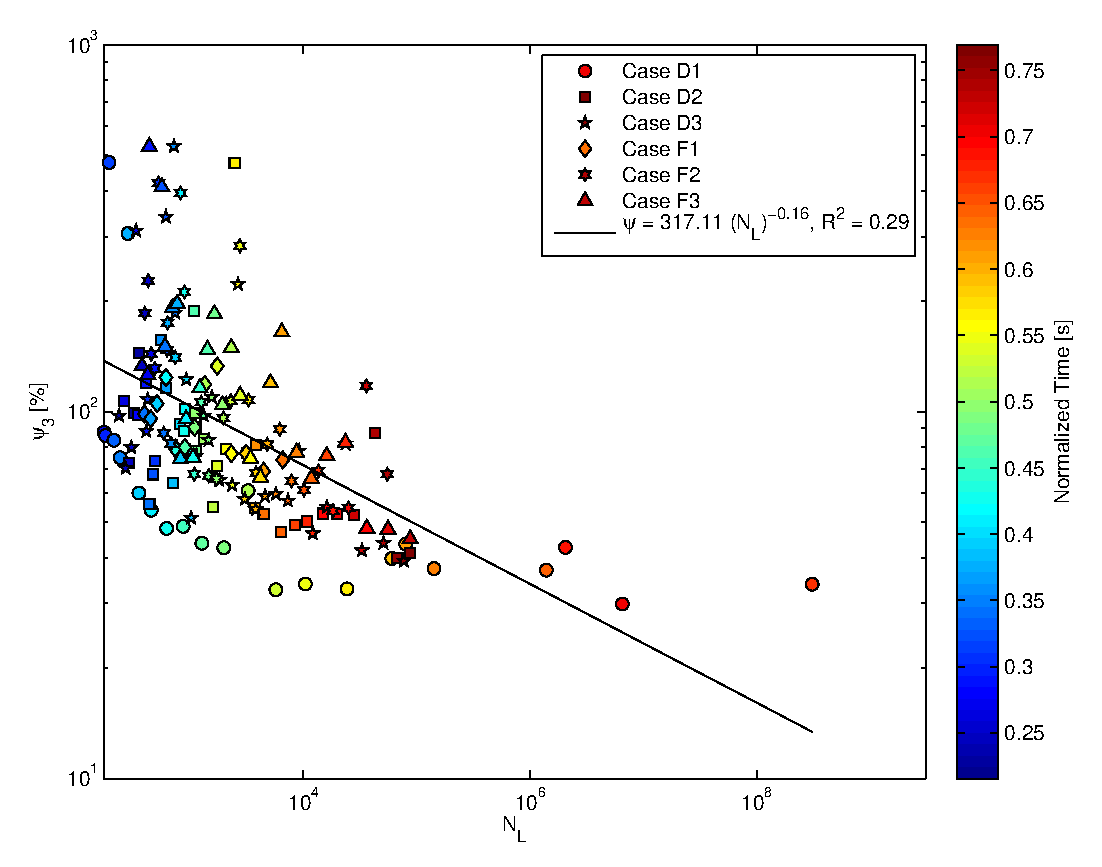
\includegraphics[width=0.49\textwidth]{Figures/phi3nl_phase}
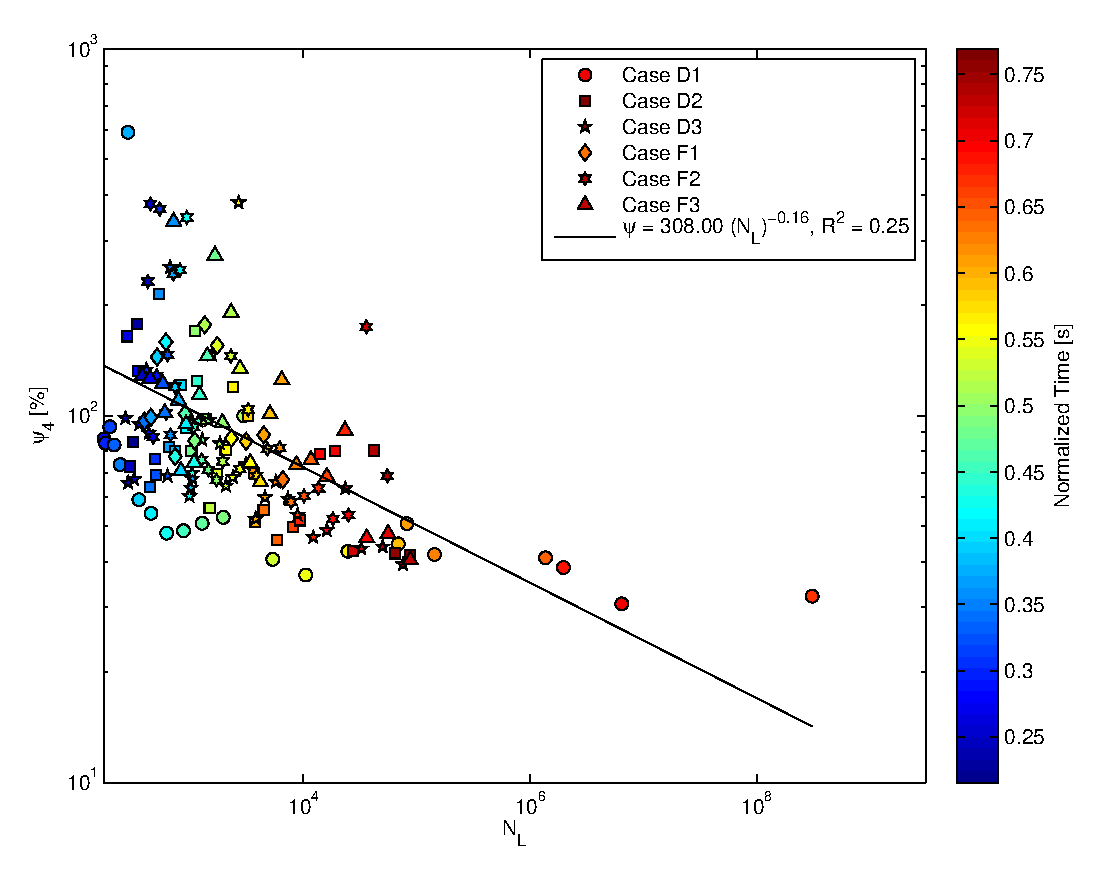
\includegraphics[width=0.49\textwidth]{Figures/phi4nl_phase}\\
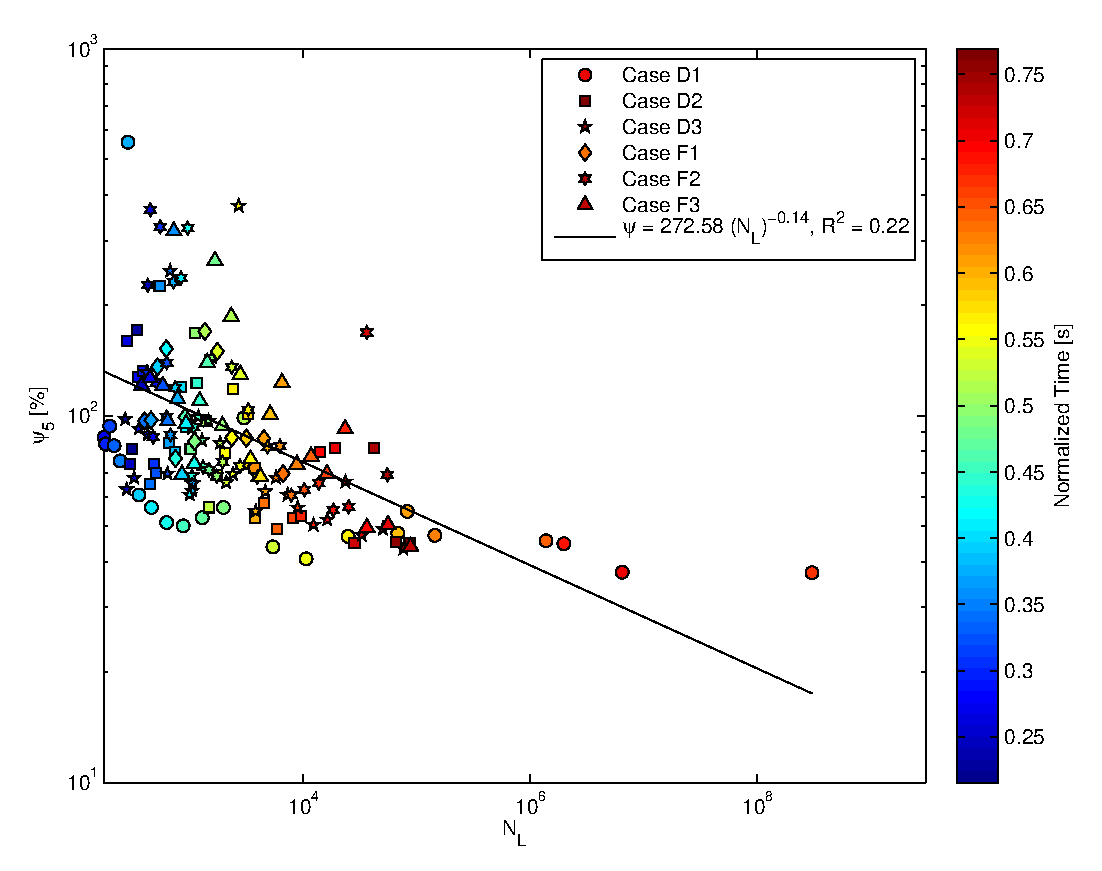
\includegraphics[width=0.49\textwidth]{Figures/phi5nl_phase}
\caption{Same as Figure 9 in the main text, but the transition scale number NL is based on
the phase relaxation time.}
\end{figure}

\begin{figure}\centering
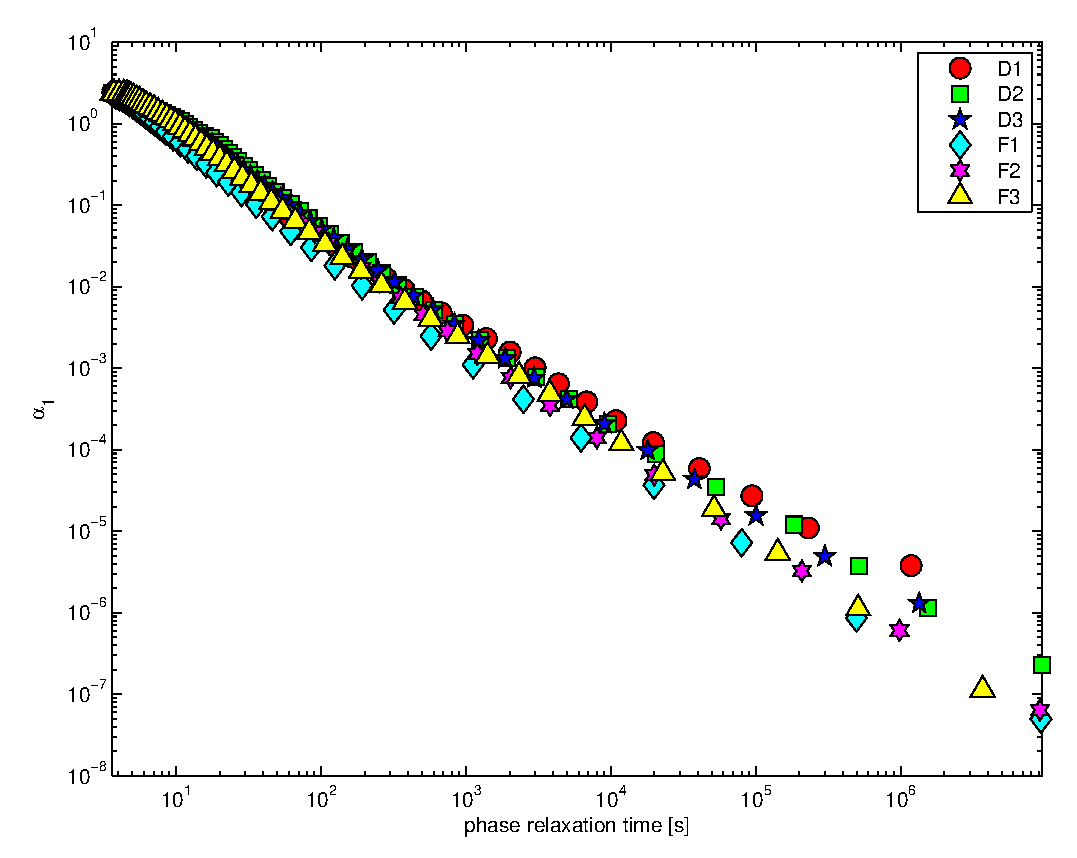
\includegraphics[width=\textwidth]{Figures/tphase_alpha}
\caption{Relationship between the prefactor $\alpha$ and phase relaxation time. The differently
colored symbols represent the six different simulation scenarios.}
\end{figure}
\end{document}